\documentclass[border=0pt]{standalone}
\usepackage[T1]{fontenc}
\usepackage{lmodern,amsmath,graphicx,tikz}
\usetikzlibrary{arrows.meta,calc,positioning}
\definecolor{ink}{HTML}{20252C}
\definecolor{blue}{HTML}{0072B2}
\definecolor{raw}{HTML}{C1272D}
\definecolor{green}{HTML}{39775A}
\definecolor{orange}{HTML}{D55E00}
\definecolor{muted}{HTML}{69717A}
\tikzset{every node/.style={font=\fontsize{9}{10.8}\selectfont,text=ink,inner sep=1mm,outer sep=0pt,align=center},
 title/.style={font=\fontsize{9}{10.8}\selectfont\bfseries},
 detail/.style={font=\fontsize{8.5}{10.2}\selectfont,text=muted},
 box/.style={draw=blue!65,fill=blue!3,line width=.65pt,rounded corners=1mm,minimum height=13mm},
 flow/.style={draw=blue,line width=.8pt,shorten <=.5pt,shorten >=.5pt,-{Latex[length=2mm,width=1.3mm]}},
 ref/.style={draw=green,dashed,line width=.7pt}}

\begin{document}
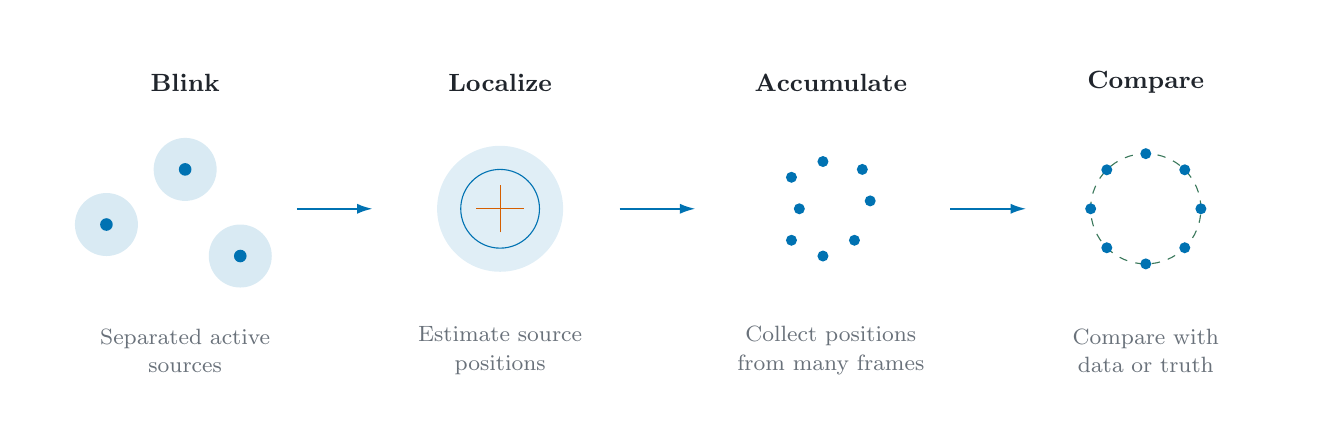
\begin{tikzpicture}[x=1mm,y=1mm]
\path[use as bounding box] (0,0) rectangle (162,48);
\foreach \x/\title/\sub in {20/Blink/{Separated active\\sources},60/Localize/{Estimate source\\positions},102/Accumulate/{Collect positions\\from many frames},142/Compare/{Compare with\\data or truth}}{
\node[title] at (\x,41) {\title};\node[detail,text width=36mm] at (\x,7) {\sub};}
\foreach \x/\y in {10/23,20/30,27/19}{\fill[blue!15] (\x,\y) circle (4mm);\fill[blue] (\x,\y) circle (.8mm);}
\fill[blue!12] (60,25) circle (8mm);\draw[blue] (60,25) circle (5mm);\draw[orange] (57,25)--(63,25) (60,22)--(60,28);
\foreach \x/\y in {97/21,98/25,97/29,101/31,106/30,107/26,105/21,101/19}{\fill[blue] (\x,\y) circle (.7mm);}
\draw[green,dashed] (142,25) circle (7mm);\foreach \a in {0,45,...,315}{\fill[blue] ($(142,25)+(\a:7mm)$) circle (.7mm);}
\foreach \a/\b in {34/44,75/85,117/127}{\draw[flow] (\a,25)--(\b,25);}
\end{tikzpicture}
\end{document}
